%%big poster size with big fonts
\documentclass[extrafontsizes, 30pt]{memoir}
\usepackage[paperheight=31in,paperwidth=47in,margin=1in,heightrounded,showframe]{geometry}

%%background from pptx
\usepackage{background}
\backgroundsetup{
scale=1,
angle=0,
opacity=1,  %% adjust
contents={\includegraphics[width=\paperwidth,height=\paperheight]{images/poster_background.pdf}}
}

%%put words where I want
\usepackage[absolute, overlay]{textpos}
\setlength{\TPHorizModule}{1in}
\setlength{\TPVertModule}{\TPHorizModule}

%%tikz setup
\usepackage{tikz, subfig, amsthm}
\usepackage{tikz-3dplot}
\usetikzlibrary{arrows, shapes, positioning, backgrounds, decorations.pathreplacing}


%%other options
\definecolor{isublue}{RGB}{58,117,196}
\definecolor{isured}{RGB}{206,17,38}
\definecolor{isugreen}{RGB}{7,109,84}
\counterwithout{figure}{chapter}
\counterwithout{table}{chapter}
\usepackage{amsmath}
\setlength{\parindent}{0cm}
\def\vdotswide{\vbox{\baselineskip=20pt \lineskiplimit=0pt \kern6pt \hbox{.}\hbox{.}\hbox{.}}} 

%%big sums
\usepackage{graphicx}
\usepackage{calc}
\newlength{\depthofsumsign}
\setlength{\depthofsumsign}{\depthof{$\sum$}}
\newcommand{\nsum}[1][1.4]{% only for \displaystyle
    \mathop{%
        \raisebox
            {-#1\depthofsumsign+1\depthofsumsign}
            {\scalebox
                {#1}
                {$\displaystyle\sum$}%
            }
    }
}

\newcommand{\Nsum}[1][1.8]{% only for \displaystyle
    \mathop{%
        \raisebox
            {-#1\depthofsumsign+1\depthofsumsign}
            {\scalebox
                {#1}
                {$\displaystyle\sum$}%
            }
    }
}

%%bibliography
\usepackage[backend=bibtex]{biblatex}
\addbibresource{refs.bib}
\renewcommand*{\bibfont}{\tiny}

\begin{document}
%% For every picture that defines or uses external nodes, you'll have to
%% apply the 'remember picture' style. To avoid some typing, we'll apply
%% the style to all pictures.
%%http://www.texample.net/tikz/examples/connecting-text-and-graphics/
\tikzstyle{every picture}+=[remember picture]
\tikzstyle{na} = [baseline=-.5ex]


%%-----------------------------------------------
%%
%%Middle big box
%%
\begin{textblock}{16}(15.5, 6.71)
{\large \bfseries Restricted Boltzmann machine (RBM)}

\begin{figure}[ht]
  \centering
  \resizebox{\linewidth}{!}{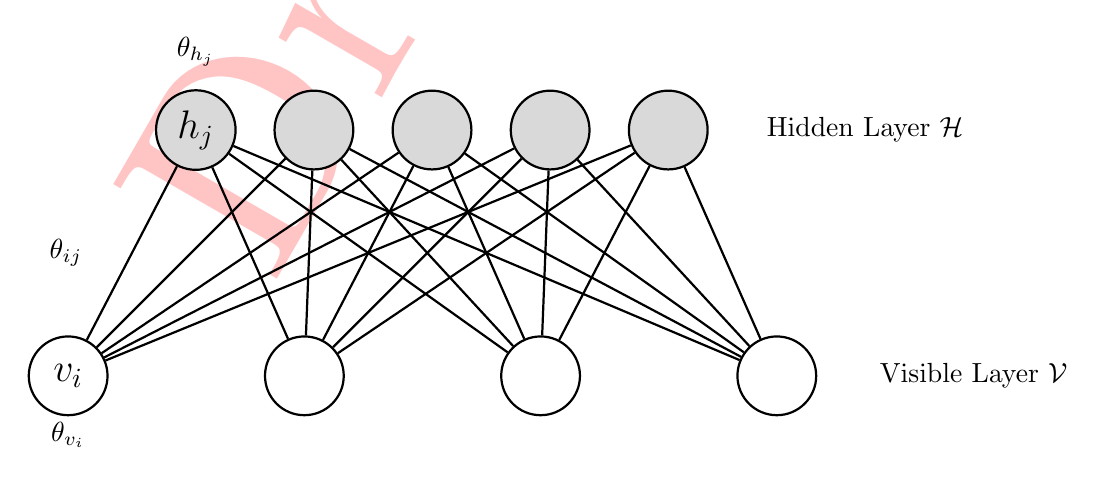
\begin{tikzpicture}[auto, node distance=3cm, thick, 
                    main node/.style= {circle,
                      fill=gray!30,
                      draw,
                      font=\sffamily\Large\bfseries,
                      minimum size=1cm}]
                      

  \node[main node] (1) {$h_j$};
  \node (11) [above of=1, yshift = -2cm] {$\theta_{h_j}$};
  \node[main node] (2) [right of=1, xshift = -1.5cm] {};
  \node[main node] (3) [right of=2, xshift = -1.5cm] {};
  \node[main node] (4) [right of=3, xshift = -1.5cm] {};
  \node[main node] (5) [right of=4, xshift = -1.5cm] {};
  \node (0) [right of=5, xshift = -.5cm] {Hidden Layer $\mathcal{H}$};
  \node[main node] (6) [below left of=1, fill=white, xshift = .5cm, yshift = -1cm] {$v_i$};
  \node (12) [below of=6, yshift = 2.25cm] {$\theta_{v_i}$};
  \node[main node] (7) [right of=6, fill=white] {};
  \node[main node] (8) [right of=7, fill=white] {};
  \node[main node] (9) [right of=8, fill=white] {};
  \node (10) [right of=9, xshift = -.5cm] {Visible Layer $\mathcal{V}$};
  
  \path
    (1) edge node [left=.5cm] {$\theta_{ij}$} (6)
        edge node {} (7)
        edge node {} (8)
        edge node {} (9)
    (2) edge node {} (6)
        edge node {} (7) 
        edge node {} (8)
        edge node {} (9)
    (3) edge node {} (6)
        edge node {} (7)
        edge node {} (8)
        edge node {} (9)
    (4) edge node {} (6)
        edge node {} (7) 
        edge node {} (8)
        edge node {} (9)
    (5) edge node {} (6)
        edge node {} (7) 
        edge node {} (8)
        edge node {} (9);
\end{tikzpicture}}
  \caption{An example restricted Boltzmann machine (RBM), which consists of two layers, a hidden ($\mathcal{H}$) and a visible layer ($\mathcal{V}$), with no connections within a layer. Hidden nodes indicated by white circles and the visible nodes indicated by blue circles \cite{friedman2001elements}.}
  \label{fig:rbm}
\end{figure}

\vspace{1cm}
\begin{figure}[ht]
  \centering
  \makeatletter
\pgfarrowsdeclare{latexnew}{latexnew}
{
  \ifdim\pgfgetarrowoptions{latexnew}=-1pt%
    \pgfutil@tempdima=0.28pt%
    \pgfutil@tempdimb=\pgflinewidth%
    \ifdim\pgfinnerlinewidth>0pt%
      \pgfmathsetlength\pgfutil@tempdimb{.6\pgflinewidth-.4*\pgfinnerlinewidth}%
    \fi%
    \advance\pgfutil@tempdima by.3\pgfutil@tempdimb%
  \else%
    \pgfutil@tempdima=\pgfgetarrowoptions{latexnew}%
    \divide\pgfutil@tempdima by 10%
  \fi%
  \pgfarrowsleftextend{+-1\pgfutil@tempdima}%
  \pgfarrowsrightextend{+9\pgfutil@tempdima}%
}
{
  \ifdim\pgfgetarrowoptions{latexnew}=-1pt%
    \pgfutil@tempdima=0.28pt%
    \pgfutil@tempdimb=\pgflinewidth%
    \ifdim\pgfinnerlinewidth>0pt%
      \pgfmathsetlength\pgfutil@tempdimb{.6\pgflinewidth-.4*\pgfinnerlinewidth}%
    \fi%
    \advance\pgfutil@tempdima by.3\pgfutil@tempdimb%
  \else%
    \pgfutil@tempdima=\pgfgetarrowoptions{latexnew}%
    \divide\pgfutil@tempdima by 10%
    \pgfsetlinewidth{0bp}%
  \fi%
  \pgfpathmoveto{\pgfqpoint{9\pgfutil@tempdima}{0pt}}
  \pgfpathcurveto
  {\pgfqpoint{6.3333\pgfutil@tempdima}{.5\pgfutil@tempdima}}
  {\pgfqpoint{2\pgfutil@tempdima}{2\pgfutil@tempdima}}
  {\pgfqpoint{-1\pgfutil@tempdima}{3.75\pgfutil@tempdima}}
  \pgfpathlineto{\pgfqpoint{-1\pgfutil@tempdima}{-3.75\pgfutil@tempdima}}
  \pgfpathcurveto
  {\pgfqpoint{2\pgfutil@tempdima}{-2\pgfutil@tempdima}}
  {\pgfqpoint{6.3333\pgfutil@tempdima}{-.5\pgfutil@tempdima}}
  {\pgfqpoint{9\pgfutil@tempdima}{0pt}}
  \pgfusepathqfill
}
\pgfsetarrowoptions{latexnew}{-1pt}
\pgfkeys{/tikz/.cd, arrowhead/.default=-1pt, arrowhead/.code={
  \pgfsetarrowoptions{latexnew}{#1}
}}

\begin{tikzpicture}[node distance=3cm, thick, 
                    visible/.style= {circle,
                      fill=isublue,
                      draw,
                      font=\Large,
                      inner sep=0pt,
                      minimum size=1cm},
                    hidden/.style= {circle,
                      fill=white,
                      draw,
                      font=\Large,
                      inner sep=0pt,
                      minimum size=1cm},
                    output/.style= {rectangle,
                    	fill=white,
                    	draw,
                    	font=\Large,
                    	inner sep=4pt,
                    	minimum size=1cm,
                    	rounded corners
                    },
                    classify/.style= {forbidden sign,
                    	fill=white,
                    	draw,
                    	font=\Large,
                    	inner sep=0pt,
                    	minimum size=2cm
                    },
                    remember picture]

    \node[anchor=north east,inner sep=0] (image) at (0,0) {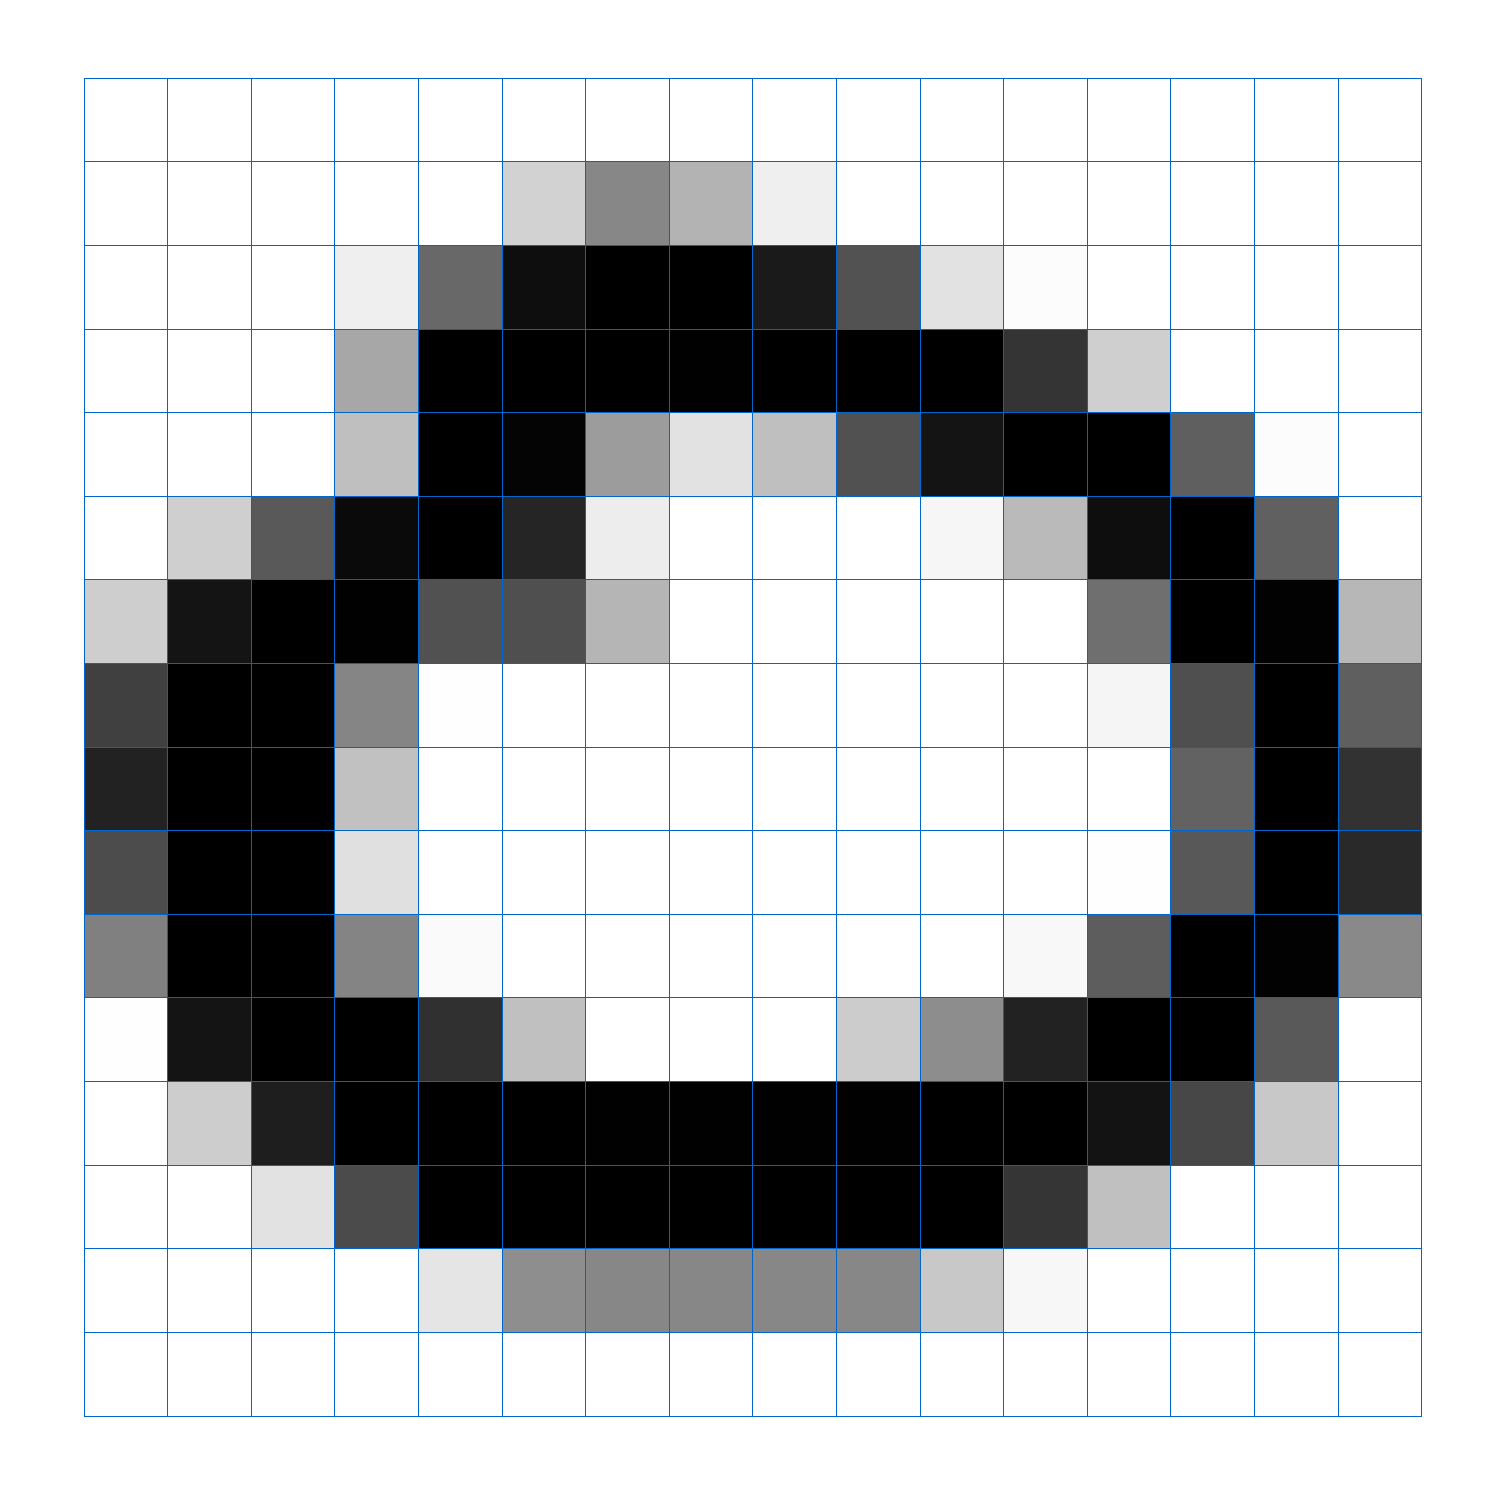
\includegraphics[height=2in]{visibles.pdf}};
    \begin{scope}[x={(image.south east)},y={(image.north west)}]
        \draw[isured, ultra thick] (0.05,0.05) rectangle (0.11,0.11);
    \end{scope}
    \node (11) [below of=image, font=\Large] {Example image};
    
	% define destination coordinates
	\path (-4.65,-.45) coordinate (first)
		  (-.45,-.45) coordinate (middle)
          (-.45,-4.65) coordinate (last);



    \node[visible] (1) [xshift = 2cm, yshift = -.8cm] {$v_1$};
    \node (2) [below of=1, yshift=2.25cm] {$\vdots$};
    \node[visible] (3) [below of=2, draw=isured, yshift=2cm] {$v_{16}$};
    \node (4) [below of=3, yshift=2.25cm] {$\vdots$};
    \node[visible] (5) [below of=4, yshift=2cm] {$v_{256}$};
    \node (12) [right of=11, xshift = 1.5cm, font=\Large] {$\mathcal{V}$};
    
    \node[hidden] (6) [right of=1] {$h_1$};
    \node(7)[below of=6, yshift=1.3cm] {$\vdotswide$};
    \node[hidden] (8) [right of=5] {$h_H$};
    %\draw [decorate, decoration={brace,amplitude=10pt}, xshift=-4pt,yshift=0pt](6,-.3) -- (6,-4.8) node (16) [black, midway, right=20pt] {};
    \draw[decoration={brace, raise=0pt, amplitude=10pt},decorate](6,-.3) -- node[right=0.5pt, midway] (16) {} (6,-4.8) ;
    
    \node (13) [right of=12, font=\Large] {$\mathcal{H}$};
    
    \node[output] (9) [right of=7, align = center, xshift=3cm] {Feature \\ representation};
    \node (14) [below of=9, font=\Large] {Output layer};
    \node[classify] (10) [right of=9, xshift=3cm, rotate=90] {};
    \node (15) [below of=10, font=\Large] {Classifier};
    
    \path
    (1) edge node {} (6)
        edge node {} (8)
    (3) edge node {} (6)
        edge node {} (8) 
    (5) edge node {} (6)
        edge node {} (8)
    (16) edge[-latexnew, arrowhead=.5cm] node {} (9)
    (9) edge[-latexnew, arrowhead=.5cm] node {} (10);
    
     \path[-latexnew, arrowhead=.5cm,black,thick] (first) edge (1);
     \path[-latexnew, arrowhead=.5cm,isured,thick] (middle) edge (3);
     \path[-latexnew, arrowhead=.5cm,black,thick] (last) edge (5);
\end{tikzpicture}

  \caption{Image classification using a RBM. On the left, each image pixel comprises a node in the visible layer, $\mathcal{V}$. On the right, the output of the RBM is used to create features which are then passed to a supervised learning algorithm.} 
  \label{fig:visibles}
\end{figure}

~\\[-1cm]
{\bfseries Joint distribution} \\[.25cm]
Let $\boldsymbol x = \{h_1, \dots, h_H, v_1,\dots,v_V\}$ represent the states of the visible and hidden nodes in an RBM. Then the probability each node taking the the value corresponding to $\boldsymbol x$ is:
\small
\begin{align}
f_{\boldsymbol \theta} (\boldsymbol x) = \frac{\exp\left(\nsum\limits_{i = 1}^V \nsum\limits_{j=1}^H \theta_{ij} v_i h_j + \nsum\limits_{i = 1}^V\theta_{v_i} v_i + \nsum\limits_{j = 1}^H\theta_{h_j} h_j\right)}{\gamma(\boldsymbol \theta)}, \quad \gamma(\boldsymbol \theta) = \Nsum\limits_{\boldsymbol x \in \mathcal{X}}\exp\left(\nsum\limits_{i = 1}^V \nsum\limits_{j=1}^H \theta_{ij} v_i h_j + \nsum\limits_{i = 1}^V\theta_{v_i} v_i + \nsum\limits_{j = 1}^H\theta_{h_j} h_j\right)
\label{eqn:pmf}
\end{align}

\end{textblock}

%%-----------------------------------------------
%%
%%Top left box
%%
\begin{textblock}{14}(.65, 5.71)
{\large \bfseries Deep learning} \\[.25cm]
\begin{minipage}{.62\textwidth}
Three layer deep Boltzmann machine, with visible-to-hidden and hidden-to-hidden connections but no within-layer connections. This can be considered as multiple single layer restricted Boltzmann machines with the lower stack hidden layer acting as the visible layer for the higher stacked model. Claimed ability to learn "internal representations that become increasingly complex" \cite{salakhutdinov2009deep}, used in classification problems.
\end{minipage}
\begin{minipage}{.38\textwidth}
\begin{figure}
  \centering
  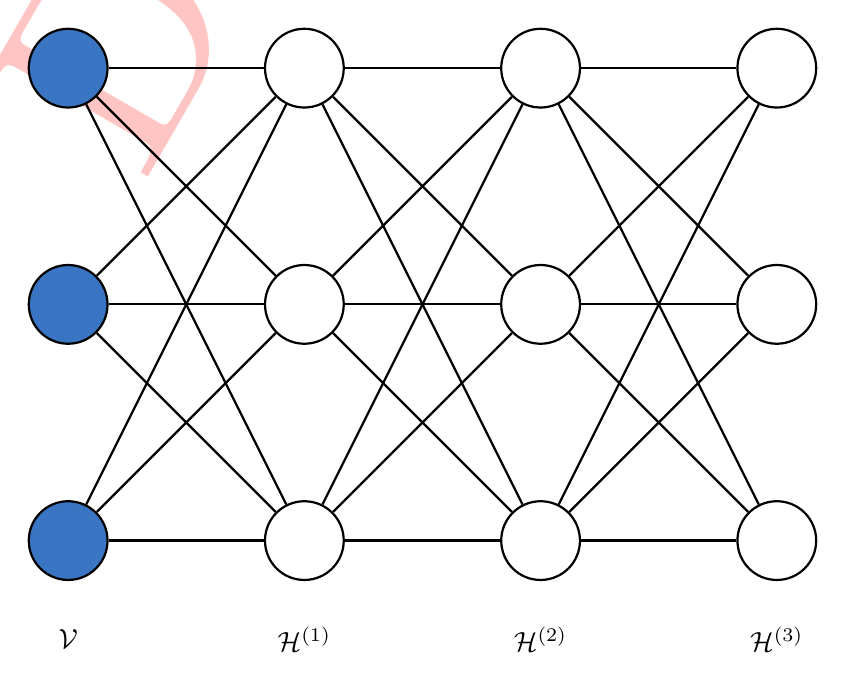
\begin{tikzpicture}[auto, node distance=3cm, thick, 
                    visible/.style= {circle,
                      fill=isublue,
                      draw,
                      font=\tiny,
                      inner sep=0pt,
                      minimum size=1cm},
                    hidden/.style= {circle,
                      fill=white,
                      draw,
                      font=\tiny,
                      inner sep=0pt,
                      minimum size=1cm}]
                      

  \node[visible] (1) {};
  \node[visible] (2) [below of=1] {};
  \node[visible] (3) [below of=2] {};
  \node (13) [below of = 3, yshift = 1.75cm] {$\mathcal{V}$};
  \node[hidden] (4) [right of=1] {};
  \node[hidden] (5) [right of=2] {};
  \node[hidden] (6) [right of=3] {};
  \node (14) [below of = 6, yshift = 1.75cm] {$\mathcal{H}^{(1)}$};
  \node[hidden] (7) [right of=4] {};
  \node[hidden] (8) [right of=5] {};
  \node[hidden] (9) [right of=6] {};
  \node (15) [below of = 9, yshift = 1.75cm] {$\mathcal{H}^{(2)}$};
  \node[hidden] (10) [right of=7] {};
  \node[hidden] (11) [right of=8] {};
  \node[hidden] (12) [right of=9] {};
  \node (16) [below of = 12, yshift = 1.75cm] {$\mathcal{H}^{(3)}$};
  
  \path
    (1) edge node {} (4)
        edge node {} (5)
        edge node {} (6)
    (2) edge node {} (4)
        edge node {} (5) 
        edge node {} (6)
    (3) edge node {} (4)
        edge node {} (5)
        edge node {} (6)
    (4) edge node {} (7)
        edge node {} (8) 
        edge node {} (9)
    (5) edge node {} (7)
        edge node {} (8) 
        edge node {} (9)
    (6) edge node {} (7)
        edge node {} (8) 
        edge node {} (9)
    (7) edge node {} (10)
        edge node {} (11) 
        edge node {} (12)
    (8) edge node {} (10)
        edge node {} (11) 
        edge node {} (12)
    (9) edge node {} (10)
        edge node {} (11) 
        edge node {} (12);
\end{tikzpicture}
  \caption{Deep RBM example.}
  \label{fig:deep_rbm}
\end{figure}
\end{minipage}


\end{textblock}

%%-----------------------------------------------
%%
%%Middle left box
%%
\begin{textblock}{14}(.65, 11.33)
{\large \bfseries Degeneracy, instability, and uninterpretability... Oh my!}\\[-1cm]

The highly flexible nature of the RBM ($H + V + HV$ parameters) makes the following characteristics of model impropriety of particular concern. \\[-.5cm]

\begin{table}
\centering
\begin{tabular}{| p{.48\linewidth} | p{.5\linewidth} |}
\hline
Characteristic & Detection \\
\hline
\hline
{\bfseries Near-degeneracy.} Occurs when there is a disproportionate amount of probability placed on only a few elements of the sample space by the model \cite{handcock2003assessing}. & If random variables in the neg-potential function $Q(\cdot)$, having support set $\mathcal{S}$, have a collective mean $\mu(\boldsymbol \theta)$ close to the boundary of the convex hull of $\mathcal{S}$. \\
%If the mean parametrization on the model parameters, $\mu(\boldsymbol \theta)$, is close to the boundary of the convex hull of the set of statistics in the neg-potential function $Q(\boldsymbol x)$. \\
\hline
{\bfseries Instability.} Small shifts in data result in large changes in probability masses, excessive sensitivity \cite{schweinberger2011instability}. & 
If, for any $c > 0$, there exists $n_c > 0$ so that $\frac{1}{V}\text{LREP}(\boldsymbol \theta) > c$ for all $V \ge n_c$, where $\text{LREP}(\boldsymbol \theta) = \log \left[\frac{\max\limits_{(v_1, \dots, v_V) \in \mathcal{X}^V}P_{\boldsymbol \theta}(v_1, \dots, v_V)}{\min\limits_{(v_1, \dots, v_V) \in \mathcal{X}^V}P_{\boldsymbol \theta}(v_1, \dots, v_V)}\right]$ \\
%If for any $C > 0$ there exists $N_C > 0$ such that  $\max\limits_{\boldsymbol x_N \in \mathcal{X}_N}[Q(\boldsymbol x_N)] > CN$ for all $N > N_C$, where $Q(\cdot)$ is the neg-potential function of the model. \\
\hline
{\bfseries Uninterpretability.} Due to the existence of dependence, marginal mean-structure no longer maintained \cite{kaiser2007statistical}. & If the magnitude of the difference between model expectations and expectations under independence (dependence parameters of zero), $\left|\text{E}(\boldsymbol X | \boldsymbol \theta) - \text{E}(\boldsymbol X | \emptyset ) \right|$, is large.\\
\hline
\end{tabular}
\label{tab:degen}
\caption{Table of ``improper model'' characteristics.}
\end{table}
\end{textblock}

%%-----------------------------------------------
%%
%%Bottom left box
%%
\begin{textblock}{14}(.65, 21.5)
{\large \bfseries Data coding to mitigate degeneracy} \\[-.75cm]

For the $\{-1, 1 \}$ encoding of $\mathcal{V}$ and $\mathcal{H}$, the origin is the center of the parameter space. In particular, at $\boldsymbol \theta = \boldsymbol 0$, the RBM is equivalent to elements of $\boldsymbol X$ being distributed as iid Bernoulli$\left(\frac{1}{2}\right)$ $\Rightarrow$ No \emph{near-degeneracy}, \emph{instability}, or \emph{uninterpretability}!
\end{textblock}
\begin{textblock}{14.5}(.65, 23.9)
%\begin{minipage}{.42\textwidth}
\begin{figure}[ht]
  \begin{minipage}{0.49\textwidth}
  \resizebox{\linewidth}{!}{
    \tdplotsetmaincoords{60}{-60}
    \tdplotsetmaincoords{60}{-60}
\begin{tikzpicture}[tdplot_main_coords, scale=1]
      \draw[dotted,->,black] (0,0,0) -- (3,0,0) node[anchor=west, font=\Large]{$x$};
      \draw[dotted,->] (0,0,0) -- (0,3,0) node[anchor=north east, font=\Large]{$y$};
      \draw[dotted,->] (0,0,0) -- (0,0,3) node[anchor=east, font=\Large]{$z$};
      
      \draw[thin,color=lightgray] (0,0,0) -- (1,0,0) -- (1,1,0) -- (0,1,0) -- (0,0,0);
      \draw[thin,color=lightgray] (0,0,0) -- (0,0,1) -- (1,0,1) -- (1,0,0) -- (0,0,0);
      \draw[thin,color=lightgray] (0,0,0) -- (0,0,1) -- (0,1,1) -- (0,1,0) -- (0,0,0);
      \draw[thin,color=lightgray] (0,0,1) -- (1,0,1) -- (1,1,1) -- (0,1,1) -- (0,0,1);
      \draw[thin,color=lightgray] (0,1,0) -- (1,1,0) -- (1,1,1) -- (0,1,1) -- (0,1,0);
      \draw[thin,color=lightgray] (1,1,0) -- (1,1,1) -- (1,0,1) -- (1,0,0) -- (1,1,0);
      
     \draw(0,1,0) -- (1,0,0) -- (0,0,0) -- (0,1,0); 
     \draw(1,1,1) -- (1,0,0) -- (0,0,0) -- (1,1,1); 
     \draw(1,1,1) -- (0,1,0) -- (0,0,0) -- (1,1,1); 
     \draw(1,1,1) -- (0,1,0) -- (1,0,0) -- (1,1,1); 
\end{tikzpicture}
    
    \draw(0,1,0) -- (1,0,0) -- (0,0,0) -- (0,1,0); 
     \draw(1,1,1) -- (1,0,0) -- (0,0,0) -- (1,1,1); 
     \draw(1,1,1) -- (0,1,0) -- (0,0,0) -- (1,1,1); 
     \draw(1,1,1) -- (0,1,0) -- (1,0,0) -- (1,1,1); 
    \end{tikzpicture}
  }
  \end{minipage}
  \begin{minipage}{0.49\textwidth}
  \resizebox{.8\linewidth}{!}{
    \tdplotsetmaincoords{60}{-60}
    \tdplotsetmaincoords{60}{-60}
\begin{tikzpicture}[tdplot_main_coords]
      \draw[dotted,->,black] (0,0,0) -- (3,0,0) node[anchor=west]{$x$};
      \draw[dotted,->] (0,0,0) -- (0,3,0) node[anchor=north east]{$y$};
      \draw[dotted,->] (0,0,0) -- (0,0,3) node[anchor=east]{$z$};
      
      \draw[thin,color=lightgray] (-1,-1,-1) -- (1,-1,-1) -- (1,1,-1) -- (-1,1,-1) -- (-1,-1,-1);
      \draw[thin,color=lightgray] (-1,-1,-1) -- (-1,-1,1) -- (1,-1,1) -- (1,-1,-1) -- (-1,-1,-1);
      \draw[thin,color=lightgray] (-1,-1,-1) -- (-1,-1,1) -- (-1,1,1) -- (-1,1,-1) -- (-1,-1,-1);
      \draw[thin,color=lightgray] (-1,-1,1) -- (1,-1,1) -- (1,1,1) -- (-1,1,1) -- (-1,-1,1);
      \draw[thin,color=lightgray] (-1,1,-1) -- (1,1,-1) -- (1,1,1) -- (-1,1,1) -- (-1,1,-1);
      \draw[thin,color=lightgray] (1,1,-1) -- (1,1,1) -- (1,-1,1) -- (1,-1,-1) -- (1,1,-1);
      
     \draw(-1,1,-1) -- (1,-1,-1) -- (-1,-1,-1) -- (-1,1,-1); 
     \draw(1,1,1) -- (1,-1,-1) -- (-1,-1,-1) -- (1,1,1); 
     \draw(1,1,1) -- (-1,1,-1) -- (-1,-1,-1) -- (1,1,1); 
     \draw(1,1,1) -- (-1,1,-1) -- (1,-1,-1) -- (1,1,1); 
\end{tikzpicture}
    
    \draw(-1,1,-1) -- (1,-1,-1) -- (-1,-1,-1) -- (-1,1,-1); 
     \draw(1,1,1) -- (1,-1,-1) -- (-1,-1,-1) -- (1,1,1); 
     \draw(1,1,1) -- (-1,1,-1) -- (-1,-1,-1) -- (1,1,1); 
     \draw(1,1,1) -- (-1,1,-1) -- (1,-1,-1) -- (1,1,1); 
    \end{tikzpicture}
  }
  \end{minipage}
  \caption{The convex hulls of the statistic space in three dimensions for a toy RBM with $|\mathcal{V}| = |\mathcal{H}| = 1$ for $\{0,1\}$-encoding (left) and $\{-1,1\}$-encoding (right) enclosed by an unrestricted hull of 3-space.}
 \label{fig:toyhull}
\end{figure}
%\end{minipage}
%\begin{minipage}{.02\textwidth}
%\hfill
%\end{minipage}
%\begin{minipage}{.55\textwidth}
%\begin{figure}
%\centering
%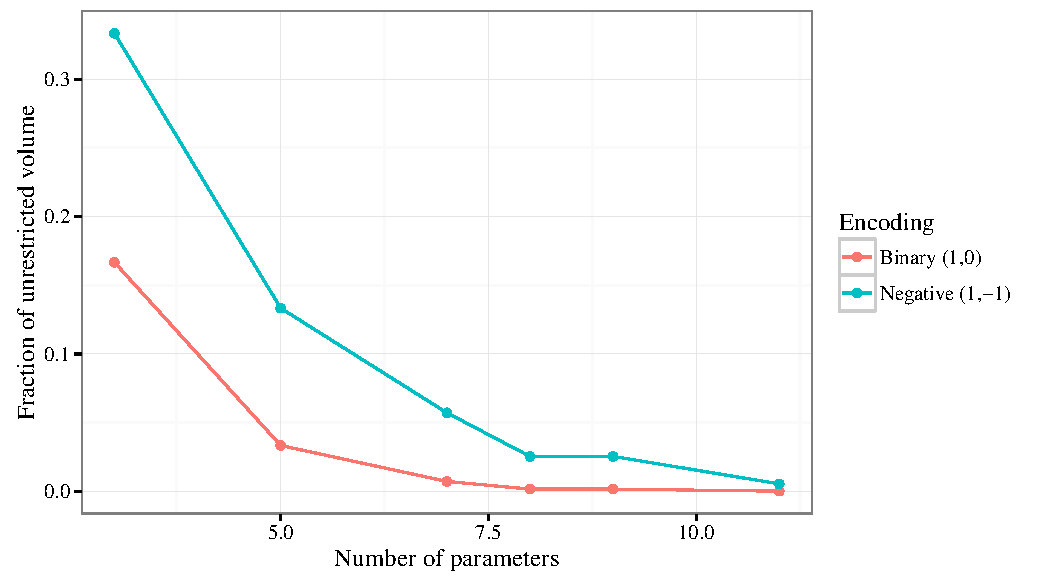
\includegraphics[scale=1]{images/frac_volume.pdf}
%\label{fig:frac_volume}
%\caption{Volume relationship for the convex hulls of statistics in $Q(\cdot)$ vs. unrestricted space.}
%\end{figure}
%\end{minipage}

\end{textblock}

%%-----------------------------------------------
%%
%%Top right box
%%
\begin{textblock}{14}(32.4, 5.71)
{\large \bfseries Manageable (a.k.a. small) examples}
\begin{figure}
\centering
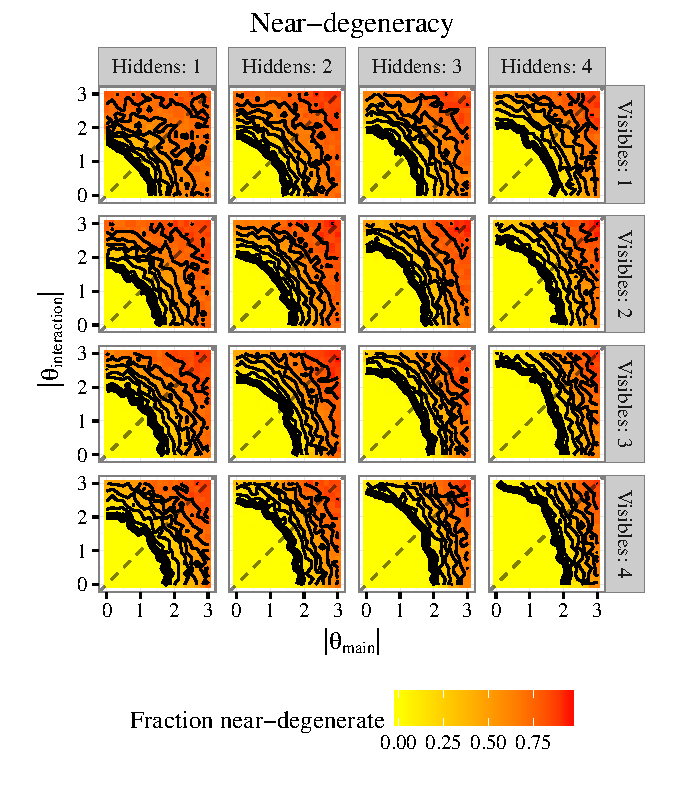
\includegraphics{images/degeneracy.pdf}
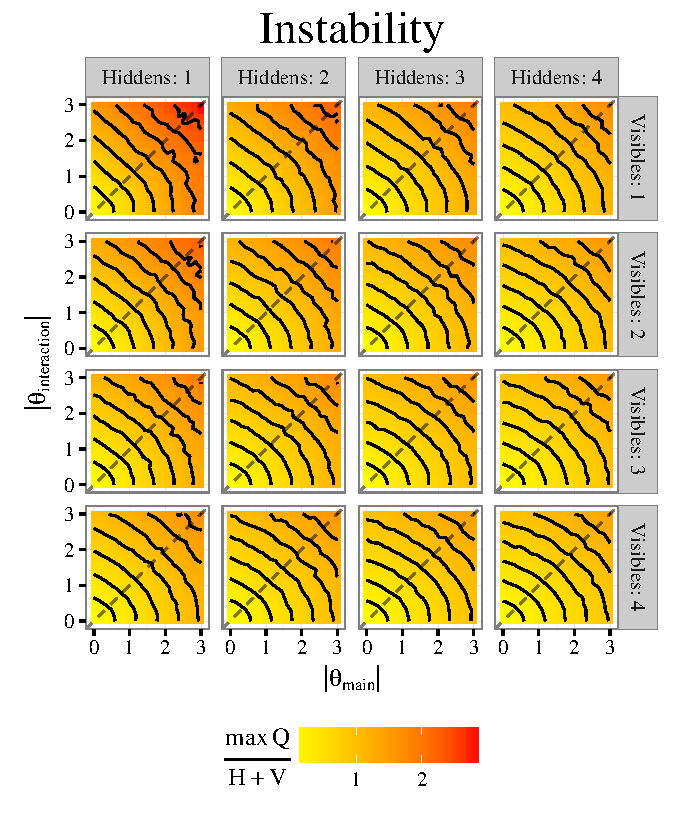
\includegraphics{images/instability.pdf}
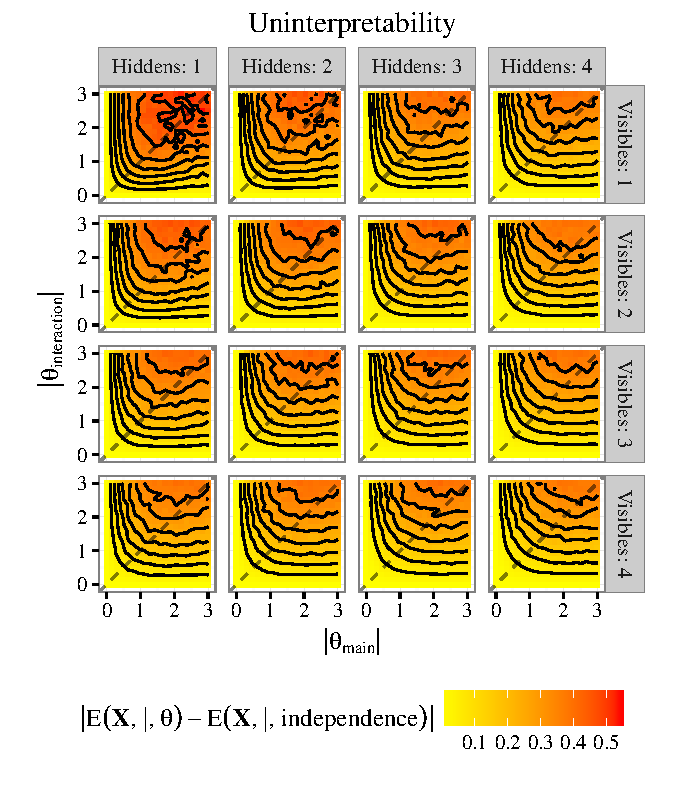
\includegraphics{images/uninterpretability.pdf}
\label{fig:three_ways}
\caption{As the magnitude of $\boldsymbol \theta$ grows ($\boldsymbol \theta$ moves from $\boldsymbol 0$), so does the occurence of near-degeneracy, instability, and uninterpretability for RBMs of varying sizes.}
\end{figure}
\end{textblock}

%%-----------------------------------------------
%%
%%Middle right box
%%
\begin{textblock}{14}(32.4, 13.8)
{\large \bfseries Bayesian model fitting} \\
{\bfseries Idea:} To avoid model impropriety, avoid parts of the parameter space that lead to \emph{near-degeneracy}, \emph{instability}, and \emph{uninterpretability} (i.e., shrink $\boldsymbol \theta$). \\[-.75cm]

Simulated $n = 5,000$ images ($V = 4, H = 4$) then fit using Bayesian methods, 
\vspace{-.5cm}
\begin{itemize}
\setlength\itemsep{.05cm}
\item {\bfseries Trick prior (BwTPLV).} Cancel out the normalizing term, full conditionals are normal. {\bfseries Conclusion:} Scalable solution, but requires tuning.
\vspace{-.75cm}
%$$\pi(\boldsymbol \theta) \propto \gamma(\boldsymbol \theta)^n \exp\left(-\frac{1}{2C_{1}}\boldsymbol \theta_{main}'\boldsymbol \theta_{main} -\frac{1}{2C_{2}}\boldsymbol \theta_{interaction}'\boldsymbol \theta_{interaction}\right) \text{\cite{li2014biclustering}}. \vspace{-.75cm}
%$$ 
\item{\bfseries Truncated Normal prior (BwTNLV).} Use two independent truncated spherical normal distributions as priors for $\theta_{main}$ and $\theta_{interaction}$ with $\sigma_{interaction} < \sigma_{main}$. Requires a geometric adaptive MH step \cite{zhou2014some} and calculation of likelihood normalizing constant. \\{\bfseries Conclusion:} Computationally intensive and convergence issues.
\item{\bfseries Marginalized likelihood (BwTNML).} Marginalize out $\boldsymbol h$ in $f_{\boldsymbol \theta}(\boldsymbol x)$, and use the truncated Normal prior. {\bfseries Conclusion:} Least scalable, but removes need to gain MCMC convergence for $Hn$ sampled hidden nodes.
\end{itemize}

\begin{figure}
\centering
\includegraphics{images/image_acf.pdf}
\label{fig:image_pred}
\vspace*{-15mm}
\caption{ACF for the posterior probabilities of each possible 4-pixel image with BwTNLV in black and BwTNML in red.}
\end{figure}

\end{textblock}

\begin{textblock}{14.54}(31.86, 25.5)
\begin{figure}
\centering
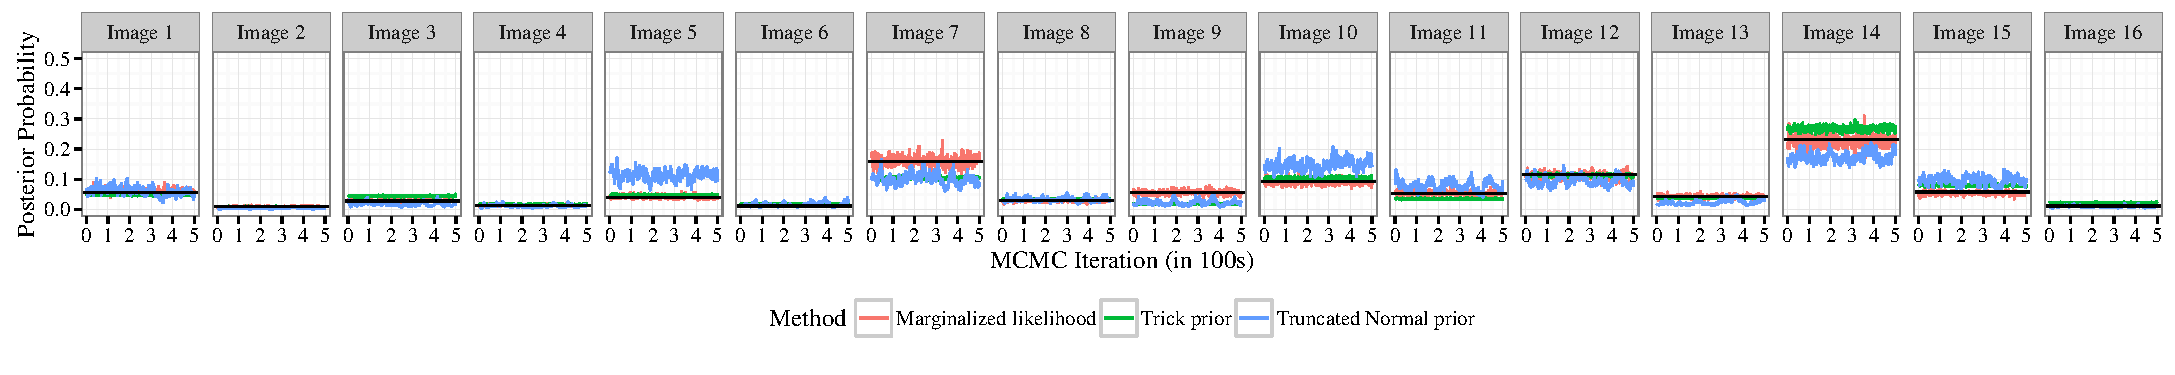
\includegraphics{images/image_prediction.pdf}
\label{fig:image_pred}
\vspace*{-15mm}
\caption{Posterior probability of each possible 4-pixel image using priors above.}
\end{figure}

{\bfseries Big takeaway:} RBMs very easily are degenerate, unstable, and uninterpretable. As compounding issues, a rigorous fitting method for these models is not scalable and merely approaches the empirical data distribution, a.k.a optimal nonparametric solution.
%only replicates the nonparametric solution (empirical distribution).
\end{textblock}

%%-----------------------------------------------
%%
%%Bottom right box
%%
%%\begin{textblock}{14}(32.4, 23.85)
%%{\large \bfseries Discussion} \\[.25cm]
%%\end{textblock}

%%\begin{textblock}{14.54}(31.86, 24.8)
%%These models very easily are degenerate, unstable, and uninterpretable. Meaning, the space of possible fitted parameter values that leads to a proper model is highly restricted.

%%To further complicate things, the proper fitting these models is very intricate and easily leads to parameter values running off to $\infty$.

%%If you're thinking of using RBMs, or stacked RBMs in a deep architecture, don't. Instead, fit a less flexible and more sensible model.

%%If you do not have an instance of every possible image in your training set, certain parameter must $\rightarrow \infty$, making fitting more complicated (shrink)

%%In reality it's practically impossible to have at least one of every possible image in your training set (large images, color scales, etc.)
%%\end{textblock}

%%-----------------------------------------------
%%
%%Bottom middle box
%%
\begin{textblock}{14.5}(16.17, 25.45)
{\large \bfseries References}
\printbibliography[heading=none]

\end{textblock}

\end{document}